\refstepcounter{section}
\section*{Lecture 04: Yang-Lee Theory for Phase Transition}
\addcontentsline{toc}{section}{Lecture 04: Yang-Lee Theory for Phase Transition}
We will now discuss about a mathematical basis of condensation based on Yang and Lee's theory of phase transition \cite{YangLee} which is based on the analysis of the zeroes of the grand partition function. The partition function seems to be an analytic function since it essentially consists of sums of well-behaved exponentials. \\[0.2cm]
However, phase transitions are characterised by non-analyticity which leads us to think about how the analytic partition function will capture the essence of the non-analytic phase transition. As discussed before, \textit{true} phase transitions occur only in the thermodynamic limit and in the thermodynamic limit, partition function can indeed become non-analytic (since the limit functions of a sequence of analytic function need not be analytic).
\subsection{Singularities and Phase Transition}
We will write Eq \eqref{eqn:gpf} in terms of the \textit{fugacity} $z=e^{\beta\mu}$ and also consider a finite system with volume $V$ (and then take ultimately take $V\to \infty$). Only a finite number of particles, say $M$, can be crammed into this finite volume, hence 
\begin{equation}
    \label{eqn:fug}
    \Xi(z,V) = \sum\limits_{N=0}^{M}z^N \SZ(N,V,T)  = 1+z\SZ_1+z^2\SZ_2+\ldots+z^M\SZ_M
\end{equation}
Note that the above equation is a well-behaved polynomial of degree $M$ in $z$  and its coefficients $\SZ_N$ are all positive which implies that $\Xi(z,V)$ has no real positive root. From the grand potential $\Phi=-PV = -\kb T\ln\Xi$, we can write the pressure $P$ and density $\rho$ in the thermodynamic limit,
\begin{align}\label{eqn:rhoP}
   \begin{split}
     P &=\lim\limits_{V\to\infty} \frac{\kb T}{V}\ln \Xi(z,V)\\
    \avg{N} &= z\pdv{\ln\Xi}{z}\implies \rho = \lim\limits_{V\to\infty} \frac{\avg{N}}{V} =\lim\limits_{V\to\infty} \frac{z}{V}\pdv{\ln\Xi(z,V)}{z}
   \end{split}
\end{align}
These quantities will not have any singularity unless $\Xi(z,V)=0$ which cannot hold true, unless we cosider a \textit{complex} fugacity. Then for finite $V$, the algebraic equation $\Xi =0$ has $M$ roots appearing in complex-conjugate pairs. As $V$ increases, the number of roots also increases (linearly with $V$) and moves around in the complex plane, excluding the real axis. In the limit $V\to\infty$, some of these roots touch the real axis and this describes a phase transition. With regard to this, we discuss two theorems as stated in the original paper.
\begin{theorem}\label{thm:1}
    For all positive values of $z$, the limit $$L = \lim\limits_{V\to\infty}\frac{1}{V}\ln\Xi(z,V)$$ \textit{exists} and is independent of the shape of the volume holding the particles, with the assumption that the surface area does not scale faster than $ V^{2/3}$. \\[0.2cm]
    Moreover, $L(z)$ is a continuous, monotonically increasing function of $z$. 
\end{theorem}

\begin{theorem}\label{thm:2}
    Suppose in the complex $z$ plane, there exists a region $\SR$ containing the positive real axis, which has no roots of $\Xi$, then $\lim\limits_{V\to \infty}\frac{1}{V}\pdv[k]{\ln \Xi}{z}$ is uniformly convergent and the limit function is analytic for all $z\in \SR$.\\[0.2cm]
    Moreover, the operations $\lim\limits_{V\to \infty}$ and $z\pdv{z}$ can be interchanged. 
\end{theorem}
The above theorem implies that, \begin{equation}\label{eqn:eos}
    \rho = \lim\limits_{V\to\infty} \frac{z}{V}\pdv{\ln\Xi}{z} \iff z\pdv{z}\qty(\lim\limits_{V\to\infty} \frac{1}{V} {\ln\Xi}) = z\pdv{(\beta P)}{z}
\end{equation}
If such a region $\SR$ does not exist, then the limit does not exist which makes sense physically, since the density $\rho $ as defined in Eq \eqref{eqn:rhoP}, does not assume a single value at the condensation point. Hence, everything depends on the existence of $\SR$
\begin{itemize}
    \item As $V\to \infty$, if a region $\SR$ exists  which fully encloses the positive real axis, then $P$ exists from Thm \eqref{thm:1} and is an analytic, increasing function of $z$. From Thm \eqref{thm:2}, $\rho$ also exists and is an analytic function of $z$. It can be shown that $\rho$ is also increasing with $z$. $P$ and $\rho$ are related by Eq \eqref{eqn:eos}. The system under consideration is in a \textit{single phase}.
    \begin{figure}[H]
        \centering
        

\tikzset{every picture/.style={line width=0.75pt}} %set default line width to 0.75pt        

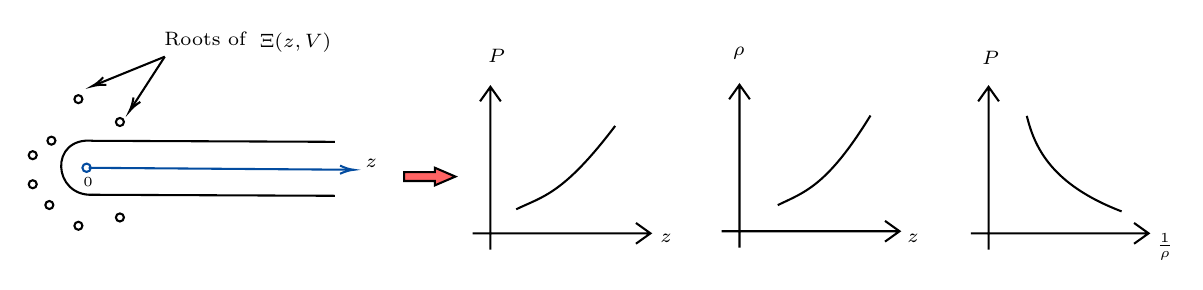
\begin{tikzpicture}[x=0.75pt,y=0.75pt,yscale=-1,xscale=1]
%uncomment if require: \path (0,300); %set diagram left start at 0, and has height of 300

%Straight Lines [id:da4940528515677156] 
\draw [draw opacity=0]   (155.68,76.5) -- (155.68,102.5) ;
%Shape: Rectangle [id:dp36230883357433774] 
\draw  [draw opacity=0] (41,76.72) -- (157.68,76.72) -- (157.68,101.5) -- (41,101.5) -- cycle ;
%Shape: Path Data [id:dp6223432909111977] 
\draw  [draw opacity=0][fill={rgb, 255:red, 255; green, 255; blue, 255 }  ,fill opacity=1 ] (41,102) .. controls (21.68,102.97) and (19.68,73.97) .. (41,76) -- (41,102) -- cycle ;
%Curve Lines [id:da24967481083813037] 
\draw    (245,109) .. controls (257.68,102.83) and (267.68,101.83) .. (292.68,68.83) ;
%Shape: Axis 2D [id:dp38393538402950345] 
\draw  (224,120.59) -- (309.68,120.59)(232.57,50) -- (232.57,128.43) (302.68,115.59) -- (309.68,120.59) -- (302.68,125.59) (227.57,57) -- (232.57,50) -- (237.57,57)  ;
%Shape: Axis 2D [id:dp05900782754200218] 
\draw  (344,119.59) -- (429.68,119.59)(352.57,49) -- (352.57,127.43) (422.68,114.59) -- (429.68,119.59) -- (422.68,124.59) (347.57,56) -- (352.57,49) -- (357.57,56)  ;
%Shape: Axis 2D [id:dp14611866266713902] 
\draw  (464,120.59) -- (549.68,120.59)(472.57,50) -- (472.57,128.43) (542.68,115.59) -- (549.68,120.59) -- (542.68,125.59) (467.57,57) -- (472.57,50) -- (477.57,57)  ;
%Curve Lines [id:da5305986343950619] 
\draw    (371,107) .. controls (383.68,100.83) and (394.68,98.02) .. (415.68,63.83) ;
%Curve Lines [id:da9611860140268851] 
\draw    (491,64) .. controls (494.68,79.02) and (502.68,97.02) .. (536.68,110.02) ;
%Shape: Boxed Bezier Curve [id:dp052814728560263036] 
\draw    (41,76) .. controls (19.68,73.97) and (21.68,102.97) .. (41,102) ;
%Shape: Boxed Line [id:dp9257530906003534] 
\draw    (41,102) -- (157.68,102.5) ;
%Shape: Boxed Line [id:dp43001914393375706] 
\draw    (41,76) -- (157.68,76.5) ;
%Shape: Circle [id:dp42172856489072374] 
\draw   (32.12,55.94) .. controls (32.12,54.87) and (32.99,54) .. (34.06,54) .. controls (35.13,54) and (36,54.87) .. (36,55.94) .. controls (36,57.01) and (35.13,57.88) .. (34.06,57.88) .. controls (32.99,57.88) and (32.12,57.01) .. (32.12,55.94) -- cycle ;
%Shape: Circle [id:dp05760255671914116] 
\draw   (32.12,116.94) .. controls (32.12,115.87) and (32.99,115) .. (34.06,115) .. controls (35.13,115) and (36,115.87) .. (36,116.94) .. controls (36,118.01) and (35.13,118.88) .. (34.06,118.88) .. controls (32.99,118.88) and (32.12,118.01) .. (32.12,116.94) -- cycle ;
%Shape: Circle [id:dp14555140857523963] 
\draw   (52.12,66.94) .. controls (52.12,65.87) and (52.99,65) .. (54.06,65) .. controls (55.13,65) and (56,65.87) .. (56,66.94) .. controls (56,68.01) and (55.13,68.88) .. (54.06,68.88) .. controls (52.99,68.88) and (52.12,68.01) .. (52.12,66.94) -- cycle ;
%Shape: Circle [id:dp4192855921408558] 
\draw   (52.12,112.94) .. controls (52.12,111.87) and (52.99,111) .. (54.06,111) .. controls (55.13,111) and (56,111.87) .. (56,112.94) .. controls (56,114.01) and (55.13,114.88) .. (54.06,114.88) .. controls (52.99,114.88) and (52.12,114.01) .. (52.12,112.94) -- cycle ;
%Shape: Circle [id:dp5888511876878247] 
\draw   (19.12,75.94) .. controls (19.12,74.87) and (19.99,74) .. (21.06,74) .. controls (22.13,74) and (23,74.87) .. (23,75.94) .. controls (23,77.01) and (22.13,77.88) .. (21.06,77.88) .. controls (19.99,77.88) and (19.12,77.01) .. (19.12,75.94) -- cycle ;
%Shape: Circle [id:dp3309756189817893] 
\draw   (18.12,106.94) .. controls (18.12,105.87) and (18.99,105) .. (20.06,105) .. controls (21.13,105) and (22,105.87) .. (22,106.94) .. controls (22,108.01) and (21.13,108.88) .. (20.06,108.88) .. controls (18.99,108.88) and (18.12,108.01) .. (18.12,106.94) -- cycle ;
%Shape: Circle [id:dp8775847429667457] 
\draw   (10.12,96.94) .. controls (10.12,95.87) and (10.99,95) .. (12.06,95) .. controls (13.13,95) and (14,95.87) .. (14,96.94) .. controls (14,98.01) and (13.13,98.88) .. (12.06,98.88) .. controls (10.99,98.88) and (10.12,98.01) .. (10.12,96.94) -- cycle ;
%Shape: Circle [id:dp29451471272880647] 
\draw   (10.12,82.94) .. controls (10.12,81.87) and (10.99,81) .. (12.06,81) .. controls (13.13,81) and (14,81.87) .. (14,82.94) .. controls (14,84.01) and (13.13,84.88) .. (12.06,84.88) .. controls (10.99,84.88) and (10.12,84.01) .. (10.12,82.94) -- cycle ;
%Right Arrow [id:dp40332084834527593] 
\draw  [color={rgb, 255:red, 0; green, 0; blue, 0 }  ,draw opacity=1 ][fill={rgb, 255:red, 255; green, 0; blue, 0 }  ,fill opacity=0.61 ] (191,91.12) -- (205.81,91.12) -- (205.81,89) -- (215.68,93.24) -- (205.81,97.48) -- (205.81,95.36) -- (191,95.36) -- cycle ;
%Straight Lines [id:da1552252445995297] 
\draw    (75.68,35.48) -- (42.54,48.95) ;
\draw [shift={(40.68,49.7)}, rotate = 337.89] [color={rgb, 255:red, 0; green, 0; blue, 0 }  ][line width=0.75]    (6.56,-1.97) .. controls (4.17,-0.84) and (1.99,-0.18) .. (0,0) .. controls (1.99,0.18) and (4.17,0.84) .. (6.56,1.97)   ;
%Straight Lines [id:da48180249394234487] 
\draw    (75.68,35.48) -- (59.77,60.02) ;
\draw [shift={(58.68,61.7)}, rotate = 302.96] [color={rgb, 255:red, 0; green, 0; blue, 0 }  ][line width=0.75]    (6.56,-1.97) .. controls (4.17,-0.84) and (1.99,-0.18) .. (0,0) .. controls (1.99,0.18) and (4.17,0.84) .. (6.56,1.97)   ;
%Straight Lines [id:da49483572214283933] 
\draw [color={rgb, 255:red, 3; green, 76; blue, 160 }  ,draw opacity=1 ]   (39.01,89.01) -- (164.68,89.95) ;
\draw [shift={(166.68,89.97)}, rotate = 180.43] [color={rgb, 255:red, 3; green, 76; blue, 160 }  ,draw opacity=1 ][line width=0.75]    (6.56,-1.97) .. controls (4.17,-0.84) and (1.99,-0.18) .. (0,0) .. controls (1.99,0.18) and (4.17,0.84) .. (6.56,1.97)   ;
\draw [shift={(38,89)}, rotate = 0.43] [color={rgb, 255:red, 3; green, 76; blue, 160 }  ,draw opacity=1 ][line width=0.75]      (0, 0) circle [x radius= 2.01, y radius= 2.01]   ;

% Text Node
\draw (230,30.4) node [anchor=north west][inner sep=0.75pt]  [font=\scriptsize]  {$P$};
% Text Node
\draw (348,29.4) node [anchor=north west][inner sep=0.75pt]  [font=\scriptsize]  {$\rho $};
% Text Node
\draw (552,119.4) node [anchor=north west][inner sep=0.75pt]  [font=\scriptsize]  {$\frac{1}{\rho} $};
% Text Node
\draw (432,119.4) node [anchor=north west][inner sep=0.75pt]  [font=\scriptsize]  {$z$};
% Text Node
\draw (313,119.4) node [anchor=north west][inner sep=0.75pt]  [font=\scriptsize]  {$z$};
% Text Node
\draw (468,31.4) node [anchor=north west][inner sep=0.75pt]  [font=\scriptsize]  {$P$};
% Text Node
\draw (35,92.4) node [anchor=north west][inner sep=0.75pt]  [font=\tiny]  {$0$};
% Text Node
\draw (171,83.4) node [anchor=north west][inner sep=0.75pt]  [font=\scriptsize]  {$z$};
% Text Node
\draw (120,22.4) node [anchor=north west][inner sep=0.75pt]  [font=\scriptsize]  {$\Xi ( z,V)$};
% Text Node
\draw (74,22) node [anchor=north west][inner sep=0.75pt]  [font=\scriptsize] [align=left] {Roots of };
% Text Node
\draw (133,80.4) node [anchor=north west][inner sep=0.75pt]  [font=\tiny]  {$\SR$};


\end{tikzpicture}

    \end{figure}
    \noindent
    \item On the other hand, if the roots of $\Xi(z,V)$ approach some specific values $z=t_1,t_2\ldots$ on the real axis as $V\to\infty$, from the figure below, there will exist regions $\SR_1,\SR_2\ldots$ within which Thm \eqref{thm:2} will be satisfied piecewise and hence, within these regions, the system exists in a single phase as argued before. At the points $t_1, t_2\ldots$, the pressure $P$ will be continuous from Thm \eqref{thm:1}, but $\rho$ might have some non-analyticity since this does not satisfy the condition for Thm \eqref{thm:2}. The system now possess \textit{multiple phases}. 
    \begin{figure}[H]
        \centering
        

\tikzset{every picture/.style={line width=0.75pt}} %set default line width to 0.75pt        

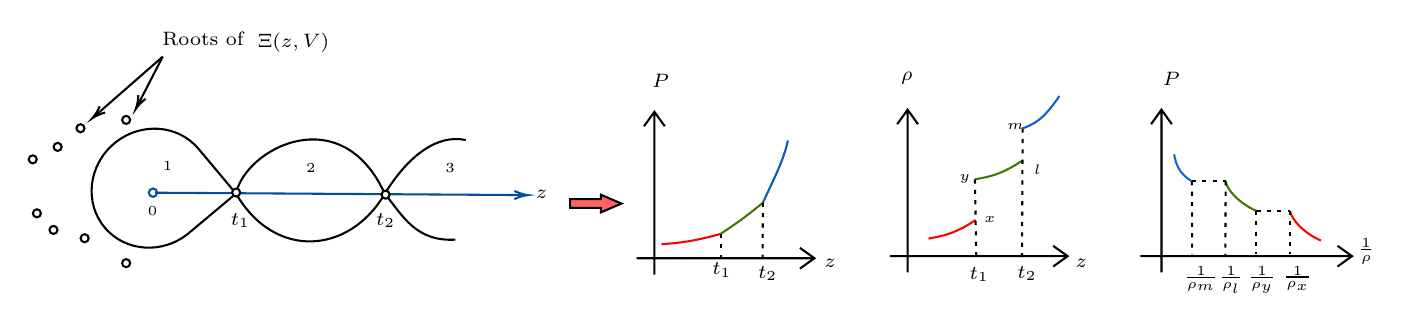
\begin{tikzpicture}[x=0.75pt,y=0.75pt,yscale=-1,xscale=1]
%uncomment if require: \path (0,372); %set diagram left start at 0, and has height of 372

%Shape: Boxed Bezier Curve [id:dp8816428801266158] 
\draw [color={rgb, 255:red, 255; green, 0; blue, 0 }  ,draw opacity=1 ]   (312,206.89) .. controls (319.57,206.12) and (325.54,205.99) .. (340.46,201.87) ;
%Shape: Axis 2D [id:dp16145854715037522] 
\draw  (300,213.59) -- (385.68,213.59)(308.57,143) -- (308.57,221.43) (378.68,208.59) -- (385.68,213.59) -- (378.68,218.59) (303.57,150) -- (308.57,143) -- (313.57,150)  ;
%Shape: Axis 2D [id:dp978316457425982] 
\draw  (422,212.59) -- (507.68,212.59)(430.57,142) -- (430.57,220.43) (500.68,207.59) -- (507.68,212.59) -- (500.68,217.59) (425.57,149) -- (430.57,142) -- (435.57,149)  ;
%Shape: Axis 2D [id:dp26039300590080416] 
\draw  (542.68,212.59) -- (644.68,212.59)(552.88,142) -- (552.88,220.43) (637.68,207.59) -- (644.68,212.59) -- (637.68,217.59) (547.88,149) -- (552.88,142) -- (557.88,149)  ;
%Shape: Boxed Bezier Curve [id:dp863718638776343] 
\draw [color={rgb, 255:red, 255; green, 0; blue, 0 }  ,draw opacity=1 ]   (440.66,204.11) .. controls (447.1,202.84) and (452.68,202.26) .. (463.34,195.19) ;
%Shape: Boxed Bezier Curve [id:dp4838128504636705] 
\draw [color={rgb, 255:red, 12; green, 107; blue, 216 }  ,draw opacity=1 ]   (559,163.55) .. controls (559.69,167.78) and (561.19,172.85) .. (567.56,176.52) ;
%Shape: Circle [id:dp11315515842109902] 
\draw   (30.12,150.94) .. controls (30.12,149.87) and (30.99,149) .. (32.06,149) .. controls (33.13,149) and (34,149.87) .. (34,150.94) .. controls (34,152.01) and (33.13,152.88) .. (32.06,152.88) .. controls (30.99,152.88) and (30.12,152.01) .. (30.12,150.94) -- cycle ;
%Shape: Circle [id:dp6787366031450796] 
\draw   (32.12,203.94) .. controls (32.12,202.87) and (32.99,202) .. (34.06,202) .. controls (35.13,202) and (36,202.87) .. (36,203.94) .. controls (36,205.01) and (35.13,205.88) .. (34.06,205.88) .. controls (32.99,205.88) and (32.12,205.01) .. (32.12,203.94) -- cycle ;
%Shape: Circle [id:dp7681830206540062] 
\draw   (52.12,146.94) .. controls (52.12,145.87) and (52.99,145) .. (54.06,145) .. controls (55.13,145) and (56,145.87) .. (56,146.94) .. controls (56,148.01) and (55.13,148.88) .. (54.06,148.88) .. controls (52.99,148.88) and (52.12,148.01) .. (52.12,146.94) -- cycle ;
%Shape: Circle [id:dp393998323220653] 
\draw   (52.12,215.94) .. controls (52.12,214.87) and (52.99,214) .. (54.06,214) .. controls (55.13,214) and (56,214.87) .. (56,215.94) .. controls (56,217.01) and (55.13,217.88) .. (54.06,217.88) .. controls (52.99,217.88) and (52.12,217.01) .. (52.12,215.94) -- cycle ;
%Shape: Circle [id:dp3591761889785463] 
\draw   (19.12,159.94) .. controls (19.12,158.87) and (19.99,158) .. (21.06,158) .. controls (22.13,158) and (23,158.87) .. (23,159.94) .. controls (23,161.01) and (22.13,161.88) .. (21.06,161.88) .. controls (19.99,161.88) and (19.12,161.01) .. (19.12,159.94) -- cycle ;
%Shape: Circle [id:dp448008178030871] 
\draw   (17.12,199.94) .. controls (17.12,198.87) and (17.99,198) .. (19.06,198) .. controls (20.13,198) and (21,198.87) .. (21,199.94) .. controls (21,201.01) and (20.13,201.88) .. (19.06,201.88) .. controls (17.99,201.88) and (17.12,201.01) .. (17.12,199.94) -- cycle ;
%Shape: Circle [id:dp8485667460597833] 
\draw   (9.12,191.94) .. controls (9.12,190.87) and (9.99,190) .. (11.06,190) .. controls (12.13,190) and (13,190.87) .. (13,191.94) .. controls (13,193.01) and (12.13,193.88) .. (11.06,193.88) .. controls (9.99,193.88) and (9.12,193.01) .. (9.12,191.94) -- cycle ;
%Shape: Circle [id:dp0935882432929589] 
\draw   (7.12,165.94) .. controls (7.12,164.87) and (7.99,164) .. (9.06,164) .. controls (10.13,164) and (11,164.87) .. (11,165.94) .. controls (11,167.01) and (10.13,167.88) .. (9.06,167.88) .. controls (7.99,167.88) and (7.12,167.01) .. (7.12,165.94) -- cycle ;
%Right Arrow [id:dp5160165324071785] 
\draw  [color={rgb, 255:red, 0; green, 0; blue, 0 }  ,draw opacity=1 ][fill={rgb, 255:red, 255; green, 0; blue, 0 }  ,fill opacity=0.61 ] (268,185.12) -- (282.81,185.12) -- (282.81,183) -- (292.68,187.24) -- (282.81,191.48) -- (282.81,189.36) -- (268,189.36) -- cycle ;
%Straight Lines [id:da40175091638638927] 
\draw    (71.68,116.48) -- (39.19,144.88) ;
\draw [shift={(37.68,146.2)}, rotate = 318.85] [color={rgb, 255:red, 0; green, 0; blue, 0 }  ][line width=0.75]    (6.56,-1.97) .. controls (4.17,-0.84) and (1.99,-0.18) .. (0,0) .. controls (1.99,0.18) and (4.17,0.84) .. (6.56,1.97)   ;
%Straight Lines [id:da42227604895998294] 
\draw    (71.68,116.48) -- (59.6,139.92) ;
\draw [shift={(58.68,141.7)}, rotate = 297.27] [color={rgb, 255:red, 0; green, 0; blue, 0 }  ][line width=0.75]    (6.56,-1.97) .. controls (4.17,-0.84) and (1.99,-0.18) .. (0,0) .. controls (1.99,0.18) and (4.17,0.84) .. (6.56,1.97)   ;
%Straight Lines [id:da403555006151344] 
\draw [draw opacity=0]   (178.68,169.5) -- (178.68,195.5) ;
%Shape: Rectangle [id:dp5158835307539544] 
\draw  [draw opacity=0] (64,169.72) -- (180.68,169.72) -- (180.68,194.5) -- (64,194.5) -- cycle ;
%Straight Lines [id:da34888006407657657] 
\draw [color={rgb, 255:red, 3; green, 76; blue, 160 }  ,draw opacity=1 ]   (68.01,182.01) -- (245.68,183.15) ;
\draw [shift={(247.68,183.17)}, rotate = 180.37] [color={rgb, 255:red, 3; green, 76; blue, 160 }  ,draw opacity=1 ][line width=0.75]    (6.56,-1.97) .. controls (4.17,-0.84) and (1.99,-0.18) .. (0,0) .. controls (1.99,0.18) and (4.17,0.84) .. (6.56,1.97)   ;
\draw [shift={(67,182)}, rotate = 0.37] [color={rgb, 255:red, 3; green, 76; blue, 160 }  ,draw opacity=1 ][line width=0.75]      (0, 0) circle [x radius= 2.01, y radius= 2.01]   ;
%Shape: Tear Drop [id:dp272851457137922] 
\draw   (84.37,201.37) .. controls (71.88,211.82) and (53.68,210.66) .. (43.72,198.77) .. controls (33.76,186.88) and (35.82,168.76) .. (48.31,158.3) .. controls (60.8,147.84) and (79,149) .. (88.96,160.9) .. controls (100.98,175.25) and (106.99,182.43) .. (106.99,182.43) .. controls (106.99,182.43) and (99.45,188.75) .. (84.37,201.37) -- cycle ;
%Curve Lines [id:da10060419654539787] 
\draw    (106.99,182.43) .. controls (111.68,160.63) and (157.68,136.63) .. (178.68,182.5) ;
%Curve Lines [id:da5863816426578047] 
\draw    (106.99,182.43) .. controls (125.68,214.63) and (161.68,211.63) .. (178.68,182.5) ;
%Curve Lines [id:da14753592564656481] 
\draw    (178.68,182.5) .. controls (189.68,164.63) and (203.68,153.63) .. (217.68,156.63) ;
%Curve Lines [id:da26991451847627657] 
\draw    (178.68,182.5) .. controls (187.68,193.58) and (193.68,205.58) .. (212.68,204.63) ;
%Shape: Circle [id:dp035910714470077876] 
\draw  [fill={rgb, 255:red, 255; green, 255; blue, 255 }  ,fill opacity=1 ] (105.12,181.94) .. controls (105.12,180.87) and (105.99,180) .. (107.06,180) .. controls (108.13,180) and (109,180.87) .. (109,181.94) .. controls (109,183.01) and (108.13,183.88) .. (107.06,183.88) .. controls (105.99,183.88) and (105.12,183.01) .. (105.12,181.94) -- cycle ;
%Shape: Circle [id:dp4309390960676185] 
\draw  [fill={rgb, 255:red, 255; green, 255; blue, 255 }  ,fill opacity=1 ] (177.12,182.94) .. controls (177.12,181.87) and (177.99,181) .. (179.06,181) .. controls (180.13,181) and (181,181.87) .. (181,182.94) .. controls (181,184.01) and (180.13,184.88) .. (179.06,184.88) .. controls (177.99,184.88) and (177.12,184.01) .. (177.12,182.94) -- cycle ;
%Curve Lines [id:da1800258159574435] 
\draw [color={rgb, 255:red, 65; green, 117; blue, 5 }  ,draw opacity=1 ]   (340.46,201.87) .. controls (349.68,195.72) and (353.68,192.72) .. (360.85,186.82) ;
%Shape: Boxed Bezier Curve [id:dp6921617703675862] 
\draw [color={rgb, 255:red, 65; green, 117; blue, 5 }  ,draw opacity=1 ]   (463,175.59) .. controls (469.44,174.31) and (475.02,173.73) .. (485.68,166.66) ;
%Curve Lines [id:da142472269960352] 
\draw [color={rgb, 255:red, 65; green, 117; blue, 5 }  ,draw opacity=1 ]   (583.77,176.52) .. controls (584.46,180.75) and (590.52,187.22) .. (598.62,190.79) ;
%Straight Lines [id:da7951881289244731] 
\draw  [dash pattern={on 1.5pt off 2.25pt}]  (340.46,201.87) -- (340.46,213.15) ;
%Straight Lines [id:da500933753036861] 
\draw  [dash pattern={on 1.5pt off 2.25pt}]  (463,175.59) -- (463.68,214.78) ;
%Straight Lines [id:da14975457152993088] 
\draw  [dash pattern={on 1.5pt off 2.25pt}]  (567.56,176.52) -- (583.77,176.52) ;
%Straight Lines [id:da1843463402056279] 
\draw  [dash pattern={on 1.5pt off 2.25pt}]  (583.77,176.52) -- (583.68,212.67) ;
%Straight Lines [id:da3624277033889689] 
\draw  [dash pattern={on 1.5pt off 2.25pt}]  (567.56,176.52) -- (567.68,211.67) ;
%Curve Lines [id:da2587872169692298] 
\draw [color={rgb, 255:red, 7; green, 91; blue, 189 }  ,draw opacity=1 ]   (360.85,186.82) .. controls (366.13,175.3) and (370.66,166.85) .. (372.93,156.87) ;
%Straight Lines [id:da9831398579139313] 
\draw  [dash pattern={on 1.5pt off 2.25pt}]  (360.85,186.82) -- (360.68,214.75) ;
%Shape: Boxed Bezier Curve [id:dp8024005479997904] 
\draw [color={rgb, 255:red, 12; green, 97; blue, 199 }  ,draw opacity=1 ]   (486,151.08) .. controls (491.02,148.85) and (495.37,147.83) .. (503.68,135.43) ;
%Straight Lines [id:da5086061427728615] 
\draw  [dash pattern={on 1.5pt off 2.25pt}]  (486,151.08) -- (485.68,213.32) ;
%Curve Lines [id:da6169340242913941] 
\draw [color={rgb, 255:red, 255; green, 0; blue, 0 }  ,draw opacity=1 ]   (614.83,190.79) .. controls (615.52,195.02) and (621.58,201.5) .. (629.68,205.07) ;
%Straight Lines [id:da6135488287955196] 
\draw  [dash pattern={on 1.5pt off 2.25pt}]  (598.62,190.79) -- (614.83,190.79) ;
%Straight Lines [id:da5610466287302585] 
\draw  [dash pattern={on 1.5pt off 2.25pt}]  (614.83,190.79) -- (614.83,211.55) ;
%Straight Lines [id:da4706916181477384] 
\draw  [dash pattern={on 1.5pt off 2.25pt}]  (598.62,190.79) -- (598.62,211.55) ;

% Text Node
\draw (306,123.4) node [anchor=north west][inner sep=0.75pt]  [font=\scriptsize]  {$P$};
% Text Node
\draw (426,122.4) node [anchor=north west][inner sep=0.75pt]  [font=\scriptsize]  {$\rho $};
% Text Node
\draw (646,202.4) node [anchor=north west][inner sep=0.75pt]  [font=\scriptsize]  {$\frac{1}{\rho }$};
% Text Node
\draw (510,212.4) node [anchor=north west][inner sep=0.75pt]  [font=\scriptsize]  {$z$};
% Text Node
\draw (389,212.4) node [anchor=north west][inner sep=0.75pt]  [font=\scriptsize]  {$z$};
% Text Node
\draw (552,122.4) node [anchor=north west][inner sep=0.75pt]  [font=\scriptsize]  {$P$};
% Text Node
\draw (63,187.4) node [anchor=north west][inner sep=0.75pt]  [font=\tiny]  {$0$};
% Text Node
\draw (116,103.4) node [anchor=north west][inner sep=0.75pt]  [font=\scriptsize]  {$\Xi ( z,V)$};
% Text Node
\draw (70,103) node [anchor=north west][inner sep=0.75pt]  [font=\scriptsize] [align=left] {Roots of };
% Text Node
\draw (250,179.4) node [anchor=north west][inner sep=0.75pt]  [font=\scriptsize]  {$z$};
% Text Node
\draw (70.31,165.46) node [anchor=north west][inner sep=0.75pt]  [font=\tiny]  {$\SR_{1}$};
% Text Node
\draw (139.31,166.7) node [anchor=north west][inner sep=0.75pt]  [font=\tiny]  {$\SR_{2}$};
% Text Node
\draw (206.31,166.7) node [anchor=north west][inner sep=0.75pt]  [font=\tiny]  {$\SR_{3}$};
% Text Node
\draw (103,190.4) node [anchor=north west][inner sep=0.75pt]  [font=\scriptsize]  {$t_{1}$};
% Text Node
\draw (173,190.4) node [anchor=north west][inner sep=0.75pt]  [font=\scriptsize]  {$t_{2}$};
% Text Node
\draw (335,214.4) node [anchor=north west][inner sep=0.75pt]  [font=\scriptsize]  {$t_{1}$};
% Text Node
\draw (466,191.81) node [anchor=north west][inner sep=0.75pt]  [font=\tiny]  {$x$};
% Text Node
\draw (454,171.68) node [anchor=north west][inner sep=0.75pt]  [font=\tiny]  {$y$};
% Text Node
\draw (610,215.9) node [anchor=north west][inner sep=0.75pt]  [font=\tiny]  {$\frac{1}{\rho _{x}}$};
% Text Node
\draw (357,215.87) node [anchor=north west][inner sep=0.75pt]  [font=\scriptsize]  {$t_{2}$};
% Text Node
\draw (490,167.3) node [anchor=north west][inner sep=0.75pt]  [font=\tiny]  {$l$};
% Text Node
\draw (477,147.17) node [anchor=north west][inner sep=0.75pt]  [font=\tiny]  {$m$};
% Text Node
\draw (593,216.1) node [anchor=north west][inner sep=0.75pt]  [font=\tiny]  {$\frac{1}{\rho _{y}}$};
% Text Node
\draw (579,216.1) node [anchor=north west][inner sep=0.75pt]  [font=\tiny]  {$\frac{1}{\rho _{l}}$};
% Text Node
\draw (562,216.1) node [anchor=north west][inner sep=0.75pt]  [font=\tiny]  {$\frac{1}{\rho _{m}}$};
% Text Node
\draw (459,216.4) node [anchor=north west][inner sep=0.75pt]  [font=\scriptsize]  {$t_{1}$};
% Text Node
\draw (482,215.87) node [anchor=north west][inner sep=0.75pt]  [font=\scriptsize]  {$t_{2}$};


\end{tikzpicture}

    \end{figure}
    \noindent 
    It is to be noted that the discontinuity in the density is only possible in the thermodynamic limit. For finite system, we will get a \textit{continuous crossover} due to \textit{finite-size effects}.\\[0.2cm]
    If $\pdv{P}{z}$ is discontinuous, then we have a \textit{first-order phase transition} as shown in the figure above. If $\pdv{P}{z}$ is continuous but $\pdv[2]{P}{z}$ is discontinuous, then we obtain a \textit{second-order phase transition}.
\end{itemize}  
From this discussion, we observe that the study of phase transitions can be reduced to just studying the distribution of the zeroes of the grand partition function.